\chapter{绪论}

\section{研究背景}

本文描述了一种高可拓展性文件分类管理软件的设计与开源实现,后文称“本软件”。

在本软件的开发过程中,涉及到了传统散列算法、局部敏感散列算法、粒子群优化等算法。了解有关的技术背景对本软件的设计与实现有很大的意义。

\subsection{传统散列算法}

散列函数(Hash function),又称哈希函数,是将任意大小的数据映射到固定大小值的函数。散列函数及其关联的散列表用于数据的存储和检索逻辑,以便在每次检索时以很小且几乎恒定的时间访问数据。它们需要的存储空间量仅略大于数据或记录本身所需的总空间。散列是一种时间复杂度和空间复杂度都十分低的数据访问形式,它避免了有序和无序列表和结构化树的非常量访问时间,以及直接访问大型或可变长度密钥的状态空间通常呈指数级的存储要求 \cite{wiki_hash}。

在密码学中,散列函数通常特指加密散列函数(加密哈希函数)。(加密)散列函数的目的是确保系统或数据的完整性,而且可以与数字签名相结合进行使用,从而提供身份验证和身份不可否认的功能 \cite{hash1}。散列函数应具有以下性质 \cite{hash2}:

\begin{enumerate}
    \item 均匀性。散列函数的定义域和值域的映射关系应当尽可能地均匀。对于任意一个给定的输入,其为值域中的每个散列值的概率应当大致相同。
    \item 确定性。对于给定的输入值,散列函数必须始终生成相同的散列值。
    \item 不可逆性。信息 $M$ 通过散列算法得到摘要 $S$。难以从 $S$ 得到 $M$。
    \item 唯一性。难以找到两个不同的信息,使得它们的摘要相同。
\end{enumerate}

常见的散列算法包括 MD5(Message Digest)和 SHA(Secure Hash Algorithm)等 \cite{hash3}。

\subsection{局部敏感散列算法}

局部敏感散列(locality-sensitive hashing, LSH)是一种算法技术,它不同于传统的散列技术,它的散列冲突是最大化的,而不是最小化的。它以高概率将相似的输入项“放入”相同的“桶”中,桶的数量远小于可能输入项目的范围,由于相似的项目最终会出现在相同的桶中,因此该技术可用于数据聚类和最近邻搜索 \cite{mmds}。该技术可以看作是一种降低维度的方法高维数据;高维的输入项可以下降为低维的项,同时保留项之间的相对距离关系。

感知散列是一种局部敏感散列算法,它使用指纹算法(可以视为一种高性能传统散列算法)生成多媒体的指纹。如果多媒体的特征相似,则感知散列是类似的。感知散列算法能够在散列之间建立关联,找到相似的数据 \cite{phash1}。

对于一张图片,其感知散列值通常是其离散余弦变换的结果与其平均值的比较结果压缩得到的 64 位整数 \cite{phash2}。图片之间的距离是其感知散列值的汉明距离。对于 64 位的感知散列值,在实际应用的过程中,通常认为汉明距离小于 13 的两张图片是有可能相似的 \cite{phash3}。

\subsection{粒子群优化概述}

粒子群优化(Particle Swarm Optimization, PSO),又称粒子群算法、微粒群算法。该算法是一种演化计算技术,来源于对一个简化社会模型的模拟,通过迭代尝试改进关于给定权重和度量的候选解决方案来优化问题 \cite{pso}。

粒子群优化的一个基本变体通过拥有候选解决方案(称为粒子)的种群(称为群)来工作。在每次迭代过程中,这些粒子根据一些简单的公式在搜索空间中位移,方向和距离由它们自己在搜索空间中的最优解位置以及整个群体在搜索空间中的最优解位置引导 \cite{pso2}。重复该过程,直到满足结束条件(如找到符合要求的解决方案或迭代达到一定次数)为止。

粒子群优化已经被广泛用于计算机视觉领域 \cite{psoimg1} \cite{psoimg2} \cite{psoimg3}。

\section{研究意义}

近年来,随着网络的快速发展,以及互联网公司的不断增多,人们获取信息的方式和速度发生了巨大的变化。大量的文件,尤其是数字媒体文件(例如图像、音频、视频等),成为了消费者日常生活中不可缺少的一部分,在拥有大量文件而且还不断增加的情况下,文件分类管理软件能够帮助用户提高处理信息的效率 \cite{cn51}。

本软件在帮助用户处理信息方面具有显著的效率提升作用,用户不再需要花费大量时间手动整理文件,而是可以利用软件快速完成这些繁琐的任务。这大大提高了信息处理的效率,使用户能够更快速地找到所需的文件。本软件还具备很高的可拓展性,使得用户可以根据自己的喜好和需求选择最适合自己的方式进行文件管理,进一步提高个性化的工作流程;同时,用户可以将本软件作为机器学习的训练辅助软件使用。

此外,本软件是自由软件。用户可以自由地使用、复制、研究、修改、分发本软件,有利于良好生态的形成 \cite{free}。同时,开放的源代码受所有用户监督、审阅,进一步提高了安全性,防止了用户隐私的泄露。

\section{研究现状分析}

\subsection{国内研究现状分析}

为方便美术设计相关从业者管理素材,市面上存在着诸多素材管理软件。本软件的标签功能与其具有一定的重合性。国内的素材管理软件中,占据最多市场的为 Eagle、Pixcall、Billfish,它们的主要功能是以标签的形式管理以图片为主的素材 \cite{eagle} \cite{pixcall} \cite{billfish}。这些软件都是专有软件,不开放源代码;体验完整功能需要付费获得。

在这些软件中,仅有 Eagle 同时面向海外市场 \cite{eagle_line}。同时,它也是国内最为流行的素材管理软件,既受到字节跳动、阿里、腾讯等大型互联网公司的青睐,也受个人用户的喜爱 \cite{eagle_count}。它提供了少量的私有协议 API,但是功能不够完善,且依赖于桌面端客户端 \cite{eagle_api}。

\begin{figure}[h]
    \centering
    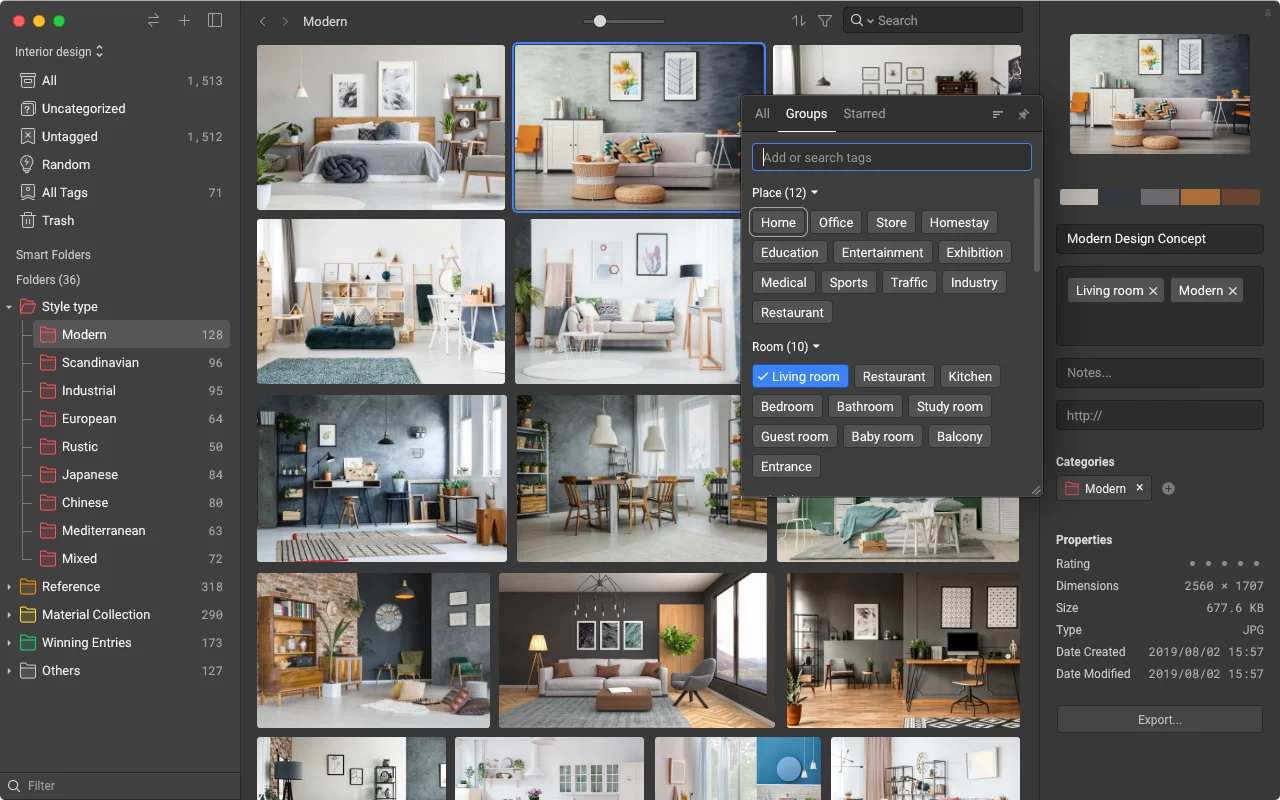
\includegraphics[width=\textwidth]{figures/eagle.png}
    \caption{Eagle 客户端界面}
    \label{fig:eagle}
\end{figure}

2022 年 09 月起至今,Eagle 用户、独立开发者 MeetQY Rao 基于 Eagle 开发了 Rao.Pics 系列开源项目 \cite{rao}。该系列开源项目实现了如下功能和特性:

\begin{enumerate}
    \item 能够读取并格式化 Eagle 的私有格式数据库。
    \item 将 Eagle 本地数据库中的内容与自己的服务器互相同步。
    \item 实现并扩充了 Eagle 的私有协议 API,并使其不需要依赖 Eagle 客户端,可以在所有具有基本的环境支持服务器上运行。
    \item 在前后端分离的架构下,基于其 API 实现了一个前端主题。该主题采用响应式布局,仿照 Eagle 客户端实现。
    \item 部署和运行可以独立于 Eagle 客户端。
\end{enumerate}

但是该系列开源项目的功能和 Eagle 客户端还具有一定的差距,且初始化过程依赖于符合 Eagle 私有格式的数据库 \cite{rao}。

\begin{figure}[h]
    \centering
    \includegraphics[width=\textwidth]{figures/rao.png}
    \caption{Rao.Pice 界面}
    \label{fig:rao}
\end{figure}

\subsection{国际研究现状分析}

国际上同样存在着许多素材管理软件,比如 Celum、Canto、Bynder 等,但它们更侧重于团队合作、交流和素材的分发 \cite{celum} \cite{canto} \cite{bynder}。这些软件也都是专有软件。

此外,与本软件功能相似的,还有自由软件 Files App、XYplorer 和 digiKam 等。

Files App 和 XYplorer 都是 Windows 文件管理器,不支持 MacOS、Linux 或其它操作系统。它们都具有选项卡式浏览、文件搜索、多功能预览、界面定制、双窗格等特性 \cite{filesapp} \cite{xyplorer}。当然,它们也各自具有独特的设计和功能。Files App 具有光滑和直观的设计,更适用于 Windows 11 \cite{filesapp}。XYplorer 具有客制化脚本的功能,可以运行用户自定义的脚本 \cite{xyplorer}。

digiKam 是一个照片管理软件,基于 XMP 查看和编辑照片的元数据,能够轻松处理大量(超过 100,000 张)图像文件 \cite{digikam}。该软件侧重于照片的浏览和处理,以及将照片发布到社交媒体上。

\begin{figure}[h]
    \centering
    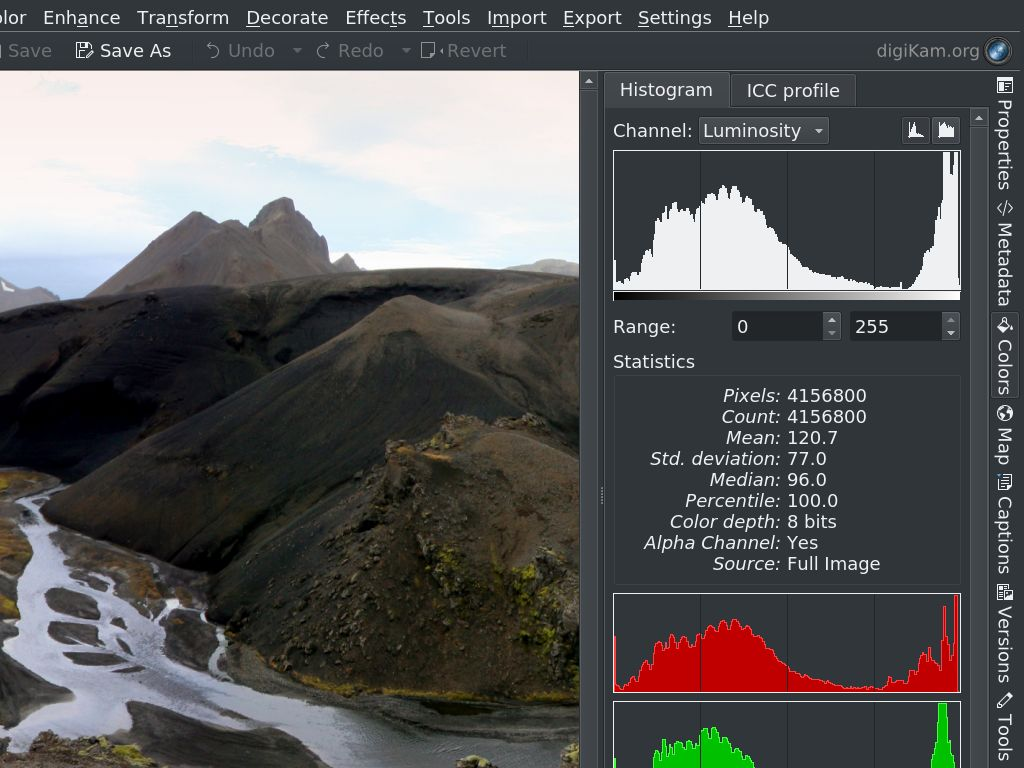
\includegraphics[width=\textwidth]{figures/digikam.jpg}
    \caption{digiKam 客户端界面}
    \label{fig:digikam}
\end{figure}

相对于上述专有软件,这些自由软件与本软件目标功能相差较大,虽然它们开放了源代码,却难以对本软件产生有效的帮助。

\section{研究思路及研究方法}

\subsection{开发流程}

依照软件工程的理论和实践经验,考虑到本软件的自由软件的性质,选择了迭代模型(Iterative model)作为软件的开发过程模型。

在开发的过程中,每次迭代遵循可行性研究、需求分析、总体设计、详细设计、编码与单元测试、集成测试等步骤,使用 Git 等工具管理代码和文档。同时,考虑到所使用的技术的掌握情况,进行了有计划的资料查阅和技能学习。

\subsection{技术方案}

在进行了可行性研究、需求分析、总体设计后,确立了如下技术方案:

\begin{enumerate}
    \item 编程语言、数据库的选择及结合方式。选择 Python 作为本软件主体部分开发语言;选择 Python 和 C++ 作为本软件插件部分开发语言;选择 SQLite 作为数据库,通过 Python 模块 sqlite3 与 Python 程序间通信。
    \item 插件系统。本软件的主体部分将只保留必要的逻辑,其中包括插件管理系统。后文中,本软件的主体部分称为“内核”。其它功能全部以插件的形式实现。
\end{enumerate}

\subsection{重难点及解决方案}

在确立了技术方案后,结合开发的实际情况,存在以下重难点,并一并提出解决方案:

\begin{enumerate}
    \item OpenCV 的编译问题。部分使用 C++ 编写的模块需要依赖 OpenCV,而对部分平台和编译器,如 Windows 上的 MinGW-W64,OpenCV 官方未直接给出相应的编译好的动态链接库 \cite{opencv_about}。因此,本文探讨了如何在 Windows 上通过 MinGW-W64 自行编译 OpenCV。
    \item 事件驱动架构(Event-driven architecture, EDA)。目前,Python 官方未支持事件驱动架构,而第三方 Python 事件驱动架构模块质量参差不齐,且大多不适合本项目 \cite{eda}。因此,本文结合 Python 的动态语言优势,提出了一种仿事件驱动的处理机制。
    \item 开源许可证冲突。本软件有大量的依赖项和参考项目,这些项目具有不同的开源许可证。如 GUN 系列软件有很多采用 GPL v2 许可证,而 OpenCV 采用 Apache 2 许可证,GPL v2 许可证与 Apache 2 许可证就是冲突的,二者不能共存 \cite{opencv_about}。因此,本文深入研究了依赖项和参考项目的开源许可证,在不引起冲突的前提下进行本软件的开发并发布源代码。
\end{enumerate}

\section{论文整体结构安排}

全文共分为 7 章,结构安排如下:

\begin{enumerate}
    \item 第 1 章:绪论。本章介绍了本软件的研究背景和研究意义,然后对研究现状进行了分析,阐述了研究思路及研究方法,及论文的整体结构安排。
    \item 第 2 章:相关概念及技术介绍。本章对本软件用到的技术和相关概念进行了介绍。
    \item 第 3 章:总体分析与设计。本章对本软件进行了可行性研究、需求分析和总体设计。
    \item 第 4 章:内核详细设计与实现。本章阐述了本软件内核及默认附加插件的详细设计和实现,包括一些常量、方法和类的定义。
    \item 第 5 章:插件详细设计与实现。本章阐述了本软件可选插件的详细设计和实现,包括一些数学、密码学、编译、算法竞赛等领域的原理。
    \item 第 6 章:测试与对比。本章对本软件测试项进行了设计,并在不同环境下对本软件进行了测试。
    \item 第 7 章:总结与展望。本章将本软件与其它相似软件进行了对比分析,对本文的研究结果和对开源社区做出了肯定和总结,分析了当前研究中的不足,规划了本软件未来的开发和维护路线,展望了本领域未来的发展。
\end{enumerate}
